\section{Segunda Parte}
\subsection{Implementaci\'on}
\subsubsection{Descripci\'on del problema}
Se pidió en esta segunda parte implementar un parser que parsee texto según la gramática especificada en la sección \ref{sec:gramatica}. Esta implementación debería tomar como entrada una cadena de texto y en caso de poder parsearla, producir como salida un archivo en formato HTML que se pueda abrir desde un browser y que dentro de él, se encuentre el texto procesado de la entrada pero correctamente indentado y coloreado.

Por ejemplo, para la siguiente entrada:

      \begin{verbatim}
<html><head><title>Título</title><script>print("hello")</script>
</head><body>texto<p>párrafo<h1><!--comentario--><p> más texto
</p></h1></p> <div>texto texto texto <br> mas texto texto texto
</div> </body> </html>\end{verbatim}

Se producirá la siguiente salida en un archivo HTML:

\begin{figure}[h!]
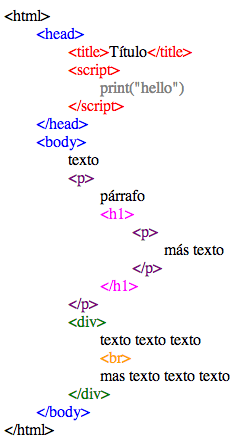
\includegraphics[width=5cm]{img/ejemplo1.png}
      \caption{Salida para un ejemplo válido.}
      \label{tbl:ejemplo}
\end{figure}

\newpage
\subsubsection{Detalles de implementación y limitaciones}


La solución fue desarrollada con ANTLR\footnote{www.antlr.org} y tanto el lexer como el parser fueron generados en Java.

El parser no acepta el símbolo \verb|<| dentro de un tag script. Esto podría tokenizarse mejor ya que una comparación dentro del script haría que falle el parsing.

En cuanto a la salida del parsing, esta es calculada en un atributo \textbf{sintetizado} llamado \texttt{texto}. Para manejar la indentación, utilizamos un único tag \verb|<div class="bloque">| cuyo único estilo tiene un margen a izquierda, fijo. El efecto de ir generando estos divs a medida que se necesita generar un tag produce la indentación deseada, contemplando el nivel de encadenamiento de tags producto de ir procesando un tag dentro de otro.

% En cuanto al coloreo de los tags, cada tag reconocido tiene su correspondiente código HTML con un estilo (CSS) que le otorga el color.
% 
% Para generar el texto del html de salida usando la gramática agregamos un atributo sintetizado de tipo \texttt{String} llamado \texttt{texto} a los símbolos no terminales. En dicho atributo se va generando el texto de salida. 

Los símbolos terminales ya poseen un atributo llamado \texttt{text} al que se accede con los métodos \texttt{getText()} y \texttt{setText()}, y que modificamos reemplazando los caracteres \texttt{<} y \texttt{>} por símbolos de escape \texttt{\&lt;} y \texttt{\&gt;} respectivamente y rodeamos de un span para darle el color adecuado. En las producciones de los símbolos no terminales sintetizamos el atributo \texttt{texto} como la concatenación de los textos de los atributos en los que produce, junto con los tags \texttt{<div>} necesarios para que se intente y coloree el texto. 

Al \texttt{texto} del símbolo distinguido \texttt{s} le agregamos también los tags \texttt{<html>}, \texttt{<head>} y \texttt{<body>} necesarios para que la salida sea un HTML válido, además de información de estilo en formato CSS.

Una modificación que debimos hacer para escribir la gramática fue pasar todos los nombres de los símbolos no terminales de mayúscula a minúscula y los de los terminales de minúscula a mayúscula. Esto se debe a que ATNLR decide si un símbolo es terminal o no terminal usando una convención inversa a la vista en clase.

\paragraph{}

Para ejecutar el programa, generamos una clase llamada \texttt{Main} que recibe por entrada estándar el HTML de entrada y genera el HTML de salida por salida estándar. Dicha clase genera un lexer usando la entrada estándar, y luego un parser usando dicho lexer. Por último ejecuta el método \texttt{s()} (correspondiente al símbolo distinguido) del parser e imprime pos salida estándar el atributo \texttt{texto}.


\paragraph{}
Un problema que tuvimos con la clase \texttt{Main} fue que si un componente interno del HTML era inválido, se reemplazaba su texto por \texttt{null}, pero el resto del archivo se imprimía normalmente. Como queremos que en caso de que la entrada no sea válida se descarte todo el HTML, decidimos sobreescribir los métodos \texttt{reportError()} del lexer y el parser. En nuestra implementación estos métodos reportan el error por \texttt{stderr} como se haría normalmente, pero además lanzan una excepción de tiempo de ejecución que interrumpe todo el programa. Modificar los métodos \texttt{reportError()} en en código de lexer y el parser traería problemas, ya que estos son autogenerados y cualquier cambio en la gramática borraría nuestra modificación; por esa razón sobreescribimos los métodos desde la clase \texttt{Main}, extendiendo el lexer y el parser.

Otro problema que tuvimos en un principio con la clase \texttt{Main} fue que ignoraba por completo los fines de línea, aceptando por ejemplo entradas donde un tag podía estar partido en varios renglones. Esto se debía a que se transformaba \texttt{stdin} en un \texttt{String}, y un bug ignoraba los fines de línea. Esto fue cambiado reemplazando el \texttt{String} por un \texttt{ANTLRInputStream} que lee directamente de la entrada.


% \newpage

\subsubsection{Entradas de prueba válidas}

\underline{Entrada 1:}
\begin{verbatim}
<html><head><title>Título</title><script>print("hello")</script>
</head><body>texto<p>párrafo<h1><!--comentario--><p> más texto
</p></h1></p> <div>texto texto texto <br> mas texto texto texto
</div> </body> </html>\end{verbatim}

\underline{Salida 1:}

\begin{figure}[h!]
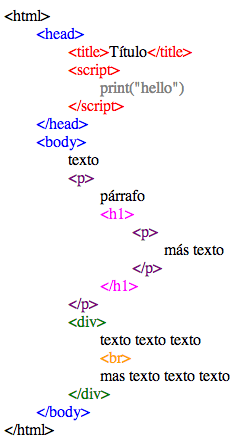
\includegraphics[width=4.7cm]{img/ejemplo1.png}
      \caption{Salida para un ejemplo válido.}
      \label{salida1}
\end{figure}

\newpage

\underline{Entrada 2:}

\begin{verbatim}
<html>  <head> <script>print("a script")</script><title>Título</title>
 <script>print("hello")</script><script>print("world")</script>
</head><body>texto suelto<p>párrafo <h1><!-- comentario--><p> más texto</p></h1>
</p><div>texto texto texto <br> mas texto textotexto</div><div>
Un Div que adentro tiene otro<div>Dentro <div><p>de otro</p> con mas texto
</div></div></div>  </body>  </html>
\end{verbatim}

\underline{Salida 2:}

\begin{figure}[h!]
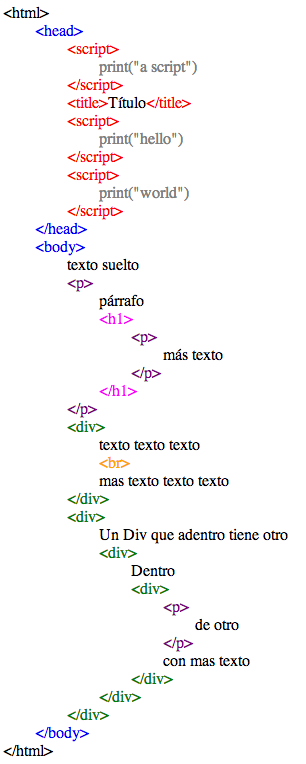
\includegraphics[width=6.2cm]{img/ejemplo2.png}
      \caption{Salida para un ejemplo válido.}
      \label{salida2}
\end{figure}

\newpage 

\subsubsection{Entradas de prueba inválidas}

\underline{Entrada 3 (\texttt{<title>} sin abrir):}
\begin{verbatim}
<html>  Título</title> <script>print("hello")</script><script>print("world")
</script></head><body>texto suelto<p>párrafo <h1><!-- comentario--><p> 
más texto</p></h1></p><div>texto texto texto <br> mas texto texto texto
</div><div>Un Div que adentro tiene otro<div>Dentro <div><p>de otro
</p> con mas texto</div></div></div></body></html>
	\end{verbatim}
    
\underline{Salida 3: (stderr)} 
\\\\
\verb|line 1:6 missing TK_C_HTML at ' Título' <html>|\\\\
\underline{Entrada 4 (\texttt{<div>} sin cerrar):}
\\\\
\begin{verbatim}
<html>  <head> <script>print("a script")</script><title>Título</title>
<script>print("hello")</script><script>print("world")</script>
</head><body>texto suelto<p>párrafo <h1><!-- comentario--><p> 
más texto</p></h1></p><div>texto texto texto <br> mas texto texto 
texto<div>Un Div que adentro tiene otro<div>Dentro <div><p>de otro</p> 
con mas texto</div></div></div></body></html>
\end{verbatim}

\underline{Salida 4: (stderr)}  \\\\
{\footnotesize
\verb|line 6:0 mismatched input '<span class="body">&lt;/body&gt;</span>' expecting TK_C_DIV|
}
